\section{System Architecture}
\label{sec:architecture}

Kura decouples model execution into two operational phases: an \textbf{Offline Physical Compilation Phase} that structures model artifacts for sequential storage streaming, and an \textbf{Online Storage-Native Serving Phase} that schedules asynchronous transfers into pre-allocated memory arenas.

\begin{figure*}[t]
\centering
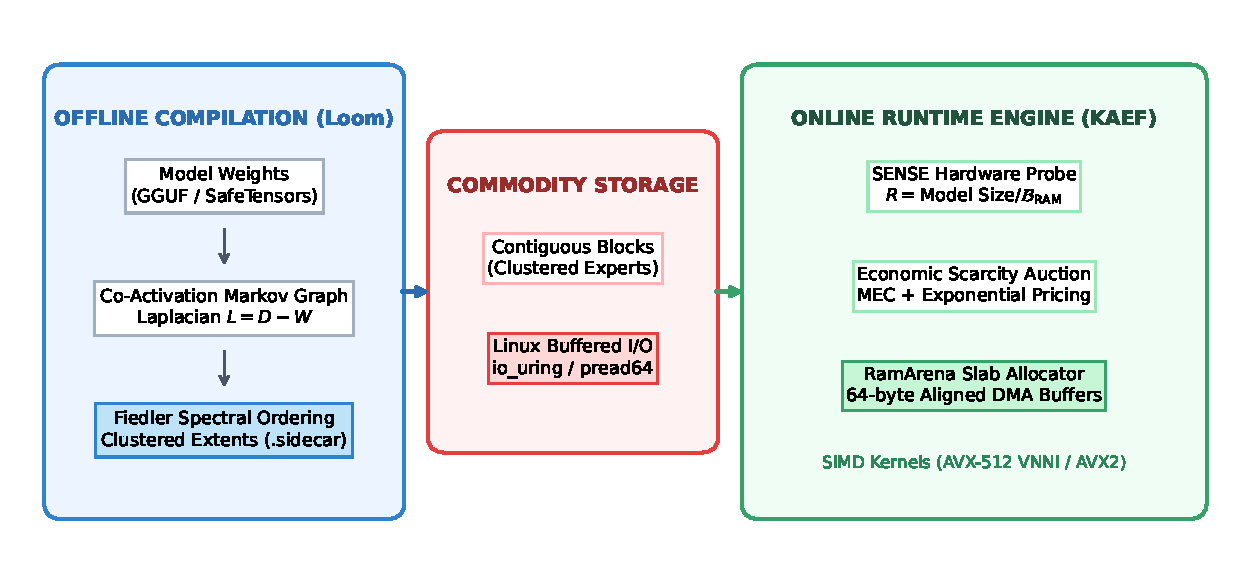
\includegraphics[width=0.92\textwidth]{figures/fig1_kura_architecture.pdf}
\caption{End-to-end Kura architecture. (1) The offline layout compiler (\textsc{Loom}) ingests model tensors and calibration traces, constructs an expert co-activation Markov graph, and writes physically clustered expert blocks to solid-state storage alongside a \texttt{.kura} layout sidecar. (2) At runtime, the hardware probe (\textsc{Sense}) benchmarks memory bandwidth, storage read rates, and core topology. (3) The execution engine schedules tensor loads using buffered asynchronous Linux \texttt{io\_uring} queues and POSIX \texttt{pread64} routines into 64-byte aligned user-space \texttt{RamArena} slabs, eliminating hot-path OS page allocations. (4) For high memory pressure, \textsc{KAEF} provides convex scarcity pricing, while precompiled \textsc{Ember} low-rank skeletons supply optional provisional draft previews.}
\label{fig:arch_overview}
\end{figure*}

\subsection{Subsystem Decomposition}
The runtime architecture consists of five modular subsystems:

\begin{enumerate}
    \item \textbf{Offline Layout Compiler (\texttt{kura-loom})}: Analyzes expert routing traces, solves the spectral arrangement heuristic, and reorders tensor byte offsets within an independent payload file without mutating original GGUF model headers.
    \item \textbf{Storage and Asynchronous I/O Layer (\texttt{kura-storage})}: Manages asynchronous kernel interactions. It implements high-concurrency \texttt{io\_uring} submission and completion ring queues, falling back to a threadpool of POSIX \texttt{pread64} workers when running on older Linux kernels.
    \item \textbf{Aligned Slab Memory Manager (\texttt{kura-memory})}: Manages physical RAM allocation via pre-allocated \texttt{RamArena} slabs. RamArena acquires a contiguous virtual memory mapping at engine initialization and sub-allocates fixed 64-byte aligned chunks for resident tensors, ensuring SIMD vector instruction alignment and preventing heap fragmentation.
    \item \textbf{Adaptive Execution Fabric (\texttt{kura-core} / \texttt{kura-econ})}: Contains the KAEF state machine. It computes marginal execution contributions, forecasts future expert routing using a Conditional Random Field (CRF), and prices memory residency using convex shadow curves. When available memory is sufficient to hold the model, KAEF is explicitly deactivated by the system classifier to eliminate scheduling overhead.
    \item \textbf{Progressive Tiered-Fidelity Engine (\texttt{kura-ember})}: Stores precompiled low-rank SVD expert sketches in a compact, permanently pinned DRAM tier, serving provisional draft representations when full weights reside on storage.
\end{enumerate}

\subsection{Memory Isolation and User-Space Buffering}
A foundational design principle of Kura is the separation of user-space memory management from the operating system's virtual memory subsystem. Standard \texttt{mmap} runtimes delegate memory management entirely to the Linux kernel, which lacks domain-specific knowledge of transformer layer sequences. Consequently, the OS kernel evicts recently loaded weights unpredictably under memory pressure.

In Kura, the memory footprint is strictly bounded by the size of the pre-allocated \texttt{RamArena}. Rather than bypassing the kernel page cache via raw buffered I/O, Kura utilizes standard buffered POSIX read calls directed into memory-pinned slab buffers. By pre-allocating the entire arena slab at initialization and managing tensor lifetimes explicitly within user-space ring buffers, Kura ensures that:
\begin{equation}
\text{RSS}_{\text{process}} \le \mathcal{B}_{\text{arena}} + \mathcal{B}_{\text{runtime\_static}}
\end{equation}
where $\mathcal{B}_{\text{arena}}$ is the user-configured RAM budget and $\mathcal{B}_{\text{runtime\_static}}$ represents the fixed overhead of token embeddings, normalization weights, and engine metadata.
